\newpage
\section{Pruebas Técnicas}

El presente capítulo describe las pruebas técnicas que se realizaron a la aplicación móvil Rem-Pills. Se verificó la funcionalidad de cada uno de los módulos y la integración de los mismos.\\

Se realizaron un total de 82 pruebas técnicas realizadas por nosotros mismos divididas en 4 ciclos de pruebas para verificar la funcionalidad de los módulos.\\

Las pruebas que se realizaron fueron pruebas de usabilidad, desempeño y disponibilidad.

Las 82 pruebas técnicas se muestran a continuación:

\subsection{Primer Ciclo de Pruebas}

Para el primer ciclo de prueba realizamos pruebas de la creación de cuentas y agregar tratamientos.

En la siguiente tabla se muestran los usuarios que fueron utilizados para el primer ciclo de pruebas:

\begin{figure}[!htbp]			
	\hypertarget{fig:Usuarios}{\hspace{1pt}}
	\begin{center}
		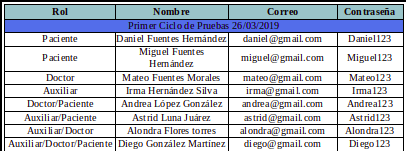
\includegraphics[height=0.3\textheight]{Pruebas/images/Usuarios1}
		\caption{Usuarios}
		\label{fig:Usuarios}
	\end{center}
\end{figure}


En la siguiente tabla se muestran los pasos que utilizamos para realizar las pruebas para el primer ciclo de pruebas:
\newpage
\begin{figure}[!htbp]			
	\hypertarget{fig:Pruebas}{\hspace{1pt}}
	\begin{center}
		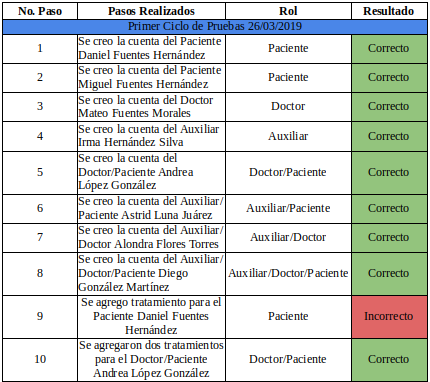
\includegraphics[height=0.5\textheight]{Pruebas/images/ppc1}
		\caption{Pruebas}
		\label{fig:Pruebas}
	\end{center}
\end{figure}

En la siguiente tabla se muestran las incidencias que resultaron durante el primer ciclo de pruebas:

\begin{figure}[!htbp]			
	\hypertarget{fig:Incidencias}{\hspace{1pt}}
	\begin{center}
		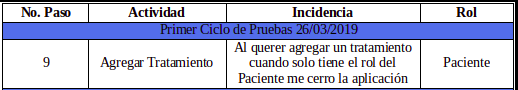
\includegraphics[height=0.1\textheight]{Pruebas/images/Inc1}
		\caption{Incidencias}
		\label{fig:Incidencias}
	\end{center}
\end{figure}

%%%%%%%%%%%%%%%%%%%%%%%%%%%%%%%%

\subsection{Segundo Ciclo de Pruebas}

Para el segundo ciclo de pruebas realizamos pruebas de creación de cuenta, agregar tratamiento, agregar medicamentos a tratamiento, agregar auxiliar y eliminar auxiliar.

En la siguiente tabla se muestran los usuarios que fueron utilizados para el segundo ciclo de pruebas:

\begin{figure}[!htbp]			
	\hypertarget{fig:usuarios2}{\hspace{1pt}}
	\begin{center}
		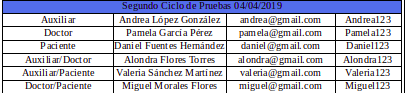
\includegraphics[height=0.17\textheight]{Pruebas/images/Usuarios2}
		\caption{Usuarios}
		\label{fig:usuarios2}
	\end{center}
\end{figure}


En la siguiente tabla se muestran los pasos que utilizamos para realizar las pruebas para el segundo ciclo de pruebas:

\begin{figure}[!htbp]			
	\hypertarget{fig:Pruebas2}{\hspace{1pt}}
	\begin{center}
		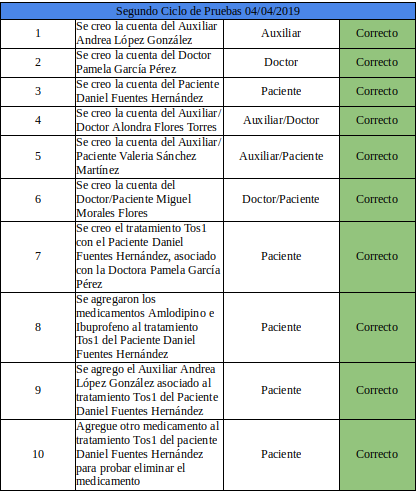
\includegraphics[height=0.4\textheight]{Pruebas/images/psc1}
		\caption{Pruebas}
		\label{fig:Pruebas2}
	\end{center}
\end{figure}
\newpage
\begin{figure}[!htbp]			
	\hypertarget{fig:Pruebas2}{\hspace{1pt}}
	\begin{center}
		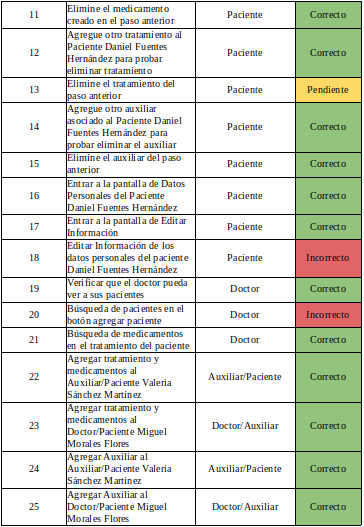
\includegraphics[height=0.4\textheight]{Pruebas/images/psc2}
		\caption{Pruebas}
		\label{fig:Pruebas2}
	\end{center}
\end{figure}

En la siguiente tabla se muestran las incidencias que resultaron durante el segundo ciclo de pruebas:

\begin{figure}[!htbp]			
	\hypertarget{fig:Incidencia2}{\hspace{1pt}}
	\begin{center}
		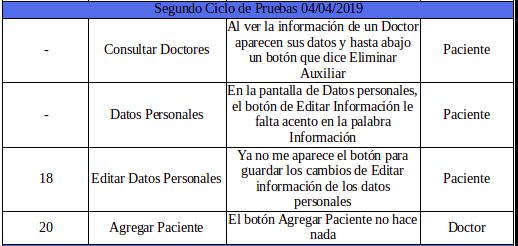
\includegraphics[height=0.3\textheight]{Pruebas/images/Inc2}
		\caption{Incidencias}
		\label{fig:Incidencia2}
	\end{center}
\end{figure}

\subsection{Tercer Ciclo de Pruebas}

Para el tercer ciclo de pruebas realizamos pruebas de creación de cuenta, agregar tratamiento, agregar medicamentos a tratamiento, agregar auxiliar y eliminar auxiliar, consulta de datos personales, y la navegación entre las pantallas de los usuarios.

En la siguiente tabla se muestran los usuarios que fueron utilizados para el tercer ciclo de pruebas:

\begin{figure}[!htbp]			
	\hypertarget{fig:usuarios3}{\hspace{1pt}}
	\begin{center}
		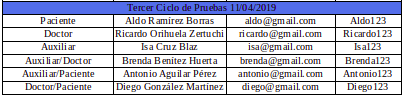
\includegraphics[height=0.17\textheight]{Pruebas/images/Usuarios3}
		\caption{Usuarios}
		\label{fig:usuarios3}
	\end{center}
\end{figure}


En la siguiente tabla se muestran los pasos que utilizamos para realizar las pruebas para el tercer ciclo de pruebas:
%\newpage

\begin{figure}[!htbp]			
	\hypertarget{fig:Pruebas3}{\hspace{1pt}}
	\begin{center}
		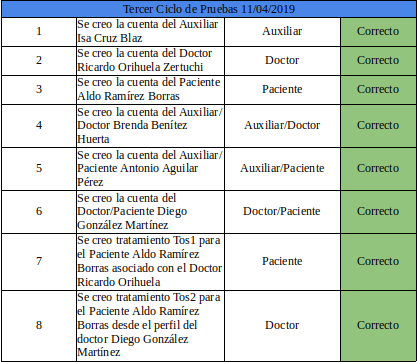
\includegraphics[height=0.35\textheight]{Pruebas/images/ptc1}
		\caption{Pruebas}
		\label{fig:Pruebas3}
	\end{center}
\end{figure}

\begin{figure}[!htbp]			
	\hypertarget{fig:Pruebas3}{\hspace{1pt}}
	\begin{center}
		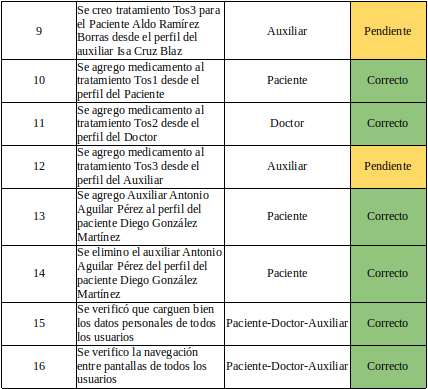
\includegraphics[height=0.35\textheight]{Pruebas/images/ptc2}
		\caption{Pruebas}
		\label{fig:Pruebas3}
	\end{center}
\end{figure}

En la siguiente tabla se muestran las incidencias que resultaron durante el tercer ciclo de pruebas:

\begin{figure}[!htbp]			
	\hypertarget{fig:Incidencia3}{\hspace{1pt}}
	\begin{center}
		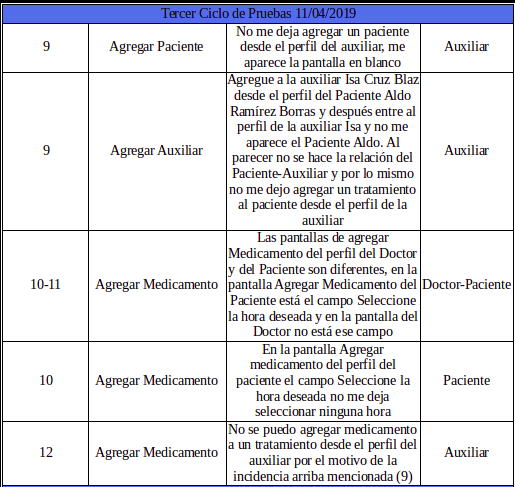
\includegraphics[height=0.35\textheight]{Pruebas/images/Inc3}
		\caption{Incidencias}
		\label{fig:Incidencia3}
	\end{center}
\end{figure}

\subsection{Cuarto Ciclo de Pruebas}

Para el cuarto ciclo de pruebas realizamos pruebas de creación de cuenta, creción de foto de perfil, validaciones de login y crear cuenta,   agregar tratamiento, agregar medicamentos a tratamiento, agregar auxiliar y eliminar auxiliar, consulta de datos personales, editar datos personales, navegación entre las pantallas de los usuario, recordatorios, realizar toma de medicamento, posponer toma de medicamento y navegación entre los roles del usuario.

En la siguiente tabla se muestran los usuarios que fueron utilizados para el cuarto ciclo de pruebas:

\begin{figure}[!htbp]			
	\hypertarget{fig:usuarios4}{\hspace{1pt}}
	\begin{center}
		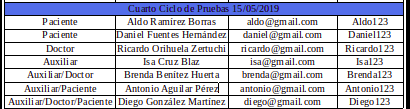
\includegraphics[height=0.17\textheight]{Pruebas/images/Usuarios4}
		\caption{Usuarios}
		\label{fig:usuarios4}
	\end{center}
\end{figure}


En la siguiente tabla se muestran los pasos que utilizamos para realizar las pruebas para el cuarto ciclo de pruebas:
\newpage

\begin{figure}[!htbp]			
	\hypertarget{fig:Pruebas4}{\hspace{1pt}}
	\begin{center}
		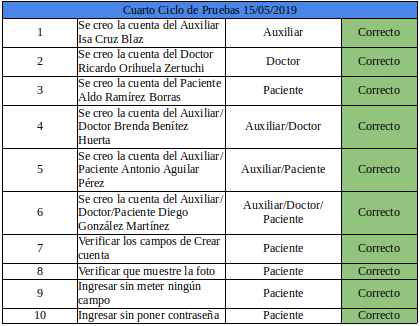
\includegraphics[height=0.35\textheight]{Pruebas/images/pcc1}
		\caption{Pruebas}
		\label{fig:Pruebas4}
	\end{center}
\end{figure}

\begin{figure}[!htbp]			
	\hypertarget{fig:Pruebas4}{\hspace{1pt}}
	\begin{center}
		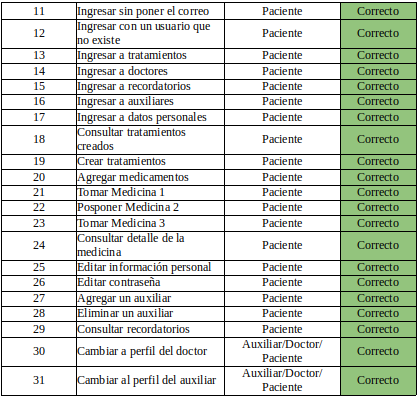
\includegraphics[height=0.4\textheight]{Pruebas/images/pcc2}
		\caption{Pruebas}
		\label{fig:Pruebas4}
	\end{center}
\end{figure}
\newpage
Para el cuarto ciclo de pruebas ya no tuvimos ninguna incidencia en cuanto al funcionamiento de los módulos de las pruebas realizadas.

%
%\subsection{Usuarios}
%
%En la siguiente tabla se muestran los usuarios que se utilizaron para realizar las pruebas durante los cuatro ciclos de prueba:
%
%\begin{figure}[!htbp]			
%	\hypertarget{fig:usuarios}{\hspace{1pt}}
%	\begin{center}
%		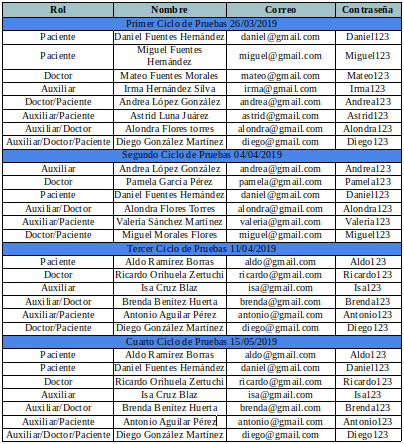
\includegraphics[height=0.5\textheight]{Pruebas/images/Usuarios}
%		\caption{Usuarios}
%		\label{fig:usuarios}
%	\end{center}
%\end{figure}
%
%\subsection{Pruebas}
%
%En la siguiente tabla se muestran los pasos que utilizamos para realizar las pruebas técnicas de la aplicación Rem-Pills.
%
%\begin{figure}[!htbp]			
%	\hypertarget{fig:Pruebas}{\hspace{1pt}}
%	\begin{center}
%		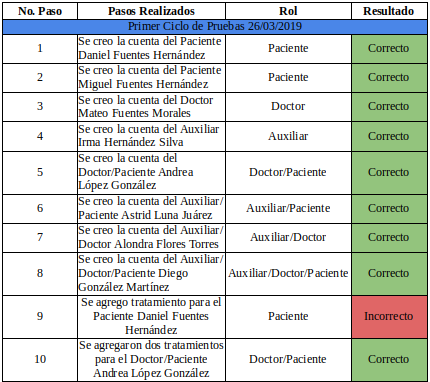
\includegraphics[height=0.7\textheight]{Pruebas/images/ppc1}
%		\caption{Pruebas}
%		\label{fig:Pruebas}
%	\end{center}
%\end{figure}
%%
%\begin{figure}[!htbp]			
%	\hypertarget{fig:Pruebas2}{\hspace{1pt}}
%	\begin{center}
%		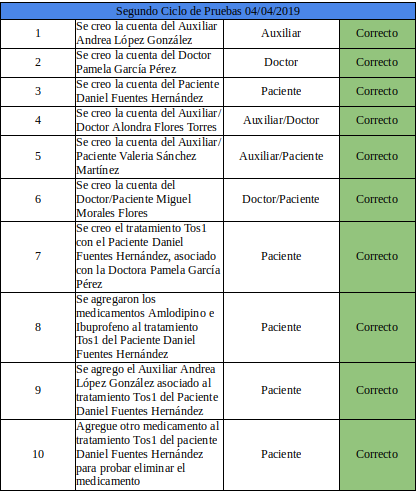
\includegraphics[height=0.8\textheight]{Pruebas/images/psc1}
%		\caption{Pruebas}
%		\label{fig:Pruebas2}
%	\end{center}
%\end{figure}
%%
%\begin{figure}[!htbp]			
%	\hypertarget{fig:Pruebas3}{\hspace{1pt}}
%	\begin{center}
%		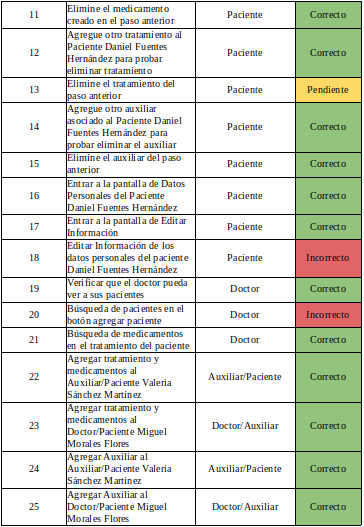
\includegraphics[height=0.9\textheight]{Pruebas/images/psc2}
%		\caption{Pruebas}
%		\label{fig:Pruebas3}
%	\end{center}
%\end{figure}
%%
%\begin{figure}[!htbp]			
%	\hypertarget{fig:Pruebas4}{\hspace{1pt}}
%	\begin{center}
%		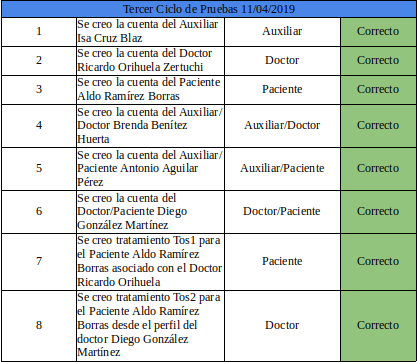
\includegraphics[height=0.67\textheight]{Pruebas/images/ptc1}
%		\caption{Pruebas}
%		\label{fig:Pruebas4}
%	\end{center}
%\end{figure}
%%\newpage
%\begin{figure}[!htbp]			
%	\hypertarget{fig:Pruebas5}{\hspace{1pt}}
%	\begin{center}
%		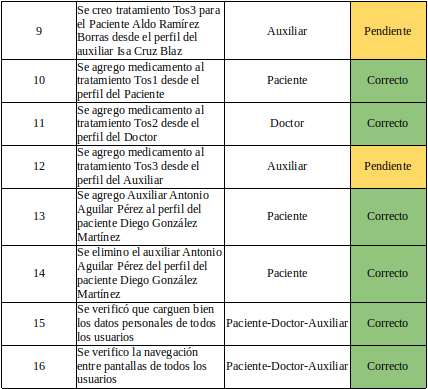
\includegraphics[height=0.7\textheight]{Pruebas/images/ptc2}
%		\caption{Pruebas}
%		\label{fig:Pruebas5}
%	\end{center}
%\end{figure}
%
%\begin{figure}[!htbp]			
%	\hypertarget{fig:Pruebas6}{\hspace{1pt}}
%	\begin{center}
%		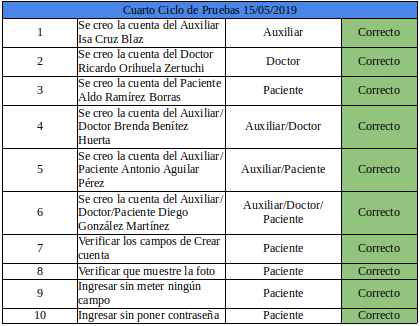
\includegraphics[height=0.6\textheight]{Pruebas/images/pcc1}
%		\caption{Pruebas}
%		\label{fig:Pruebas6}
%	\end{center}
%\end{figure}
%
%\begin{figure}[!htbp]			
%	\hypertarget{fig:Pruebas7}{\hspace{1pt}}
%	\begin{center}
%		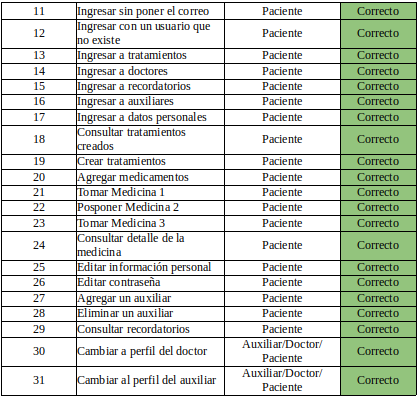
\includegraphics[height=0.75\textheight]{Pruebas/images/pcc2}
%		\caption{Pruebas}
%		\label{fig:Pruebas7}
%	\end{center}
%\end{figure}
%
%\newpage
%\subsection{Incidencias}
%
%En la siguiente tabla se muestran las incidencias que fuimos encontrando durante estos cuatro ciclos de prueba.
%%
%\begin{figure}[!htbp]			
%	\hypertarget{fig:Incidencias}{\hspace{1pt}}
%	\begin{center}
%		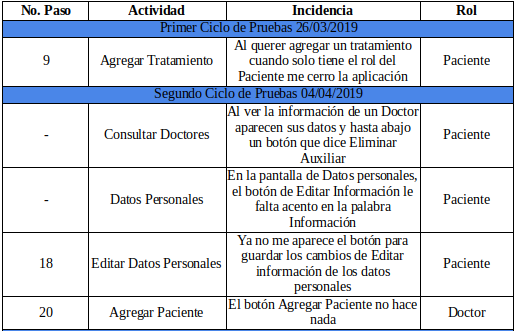
\includegraphics[height=0.5\textheight]{Pruebas/images/Inc1y2}
%		\caption{Incidencias}
%		\label{fig:Incidencias}
%	\end{center}
%\end{figure}
%
%%
%\begin{figure}[!htbp]			
%	\hypertarget{fig:Incidencias2}{\hspace{1pt}}
%	\begin{center}
%		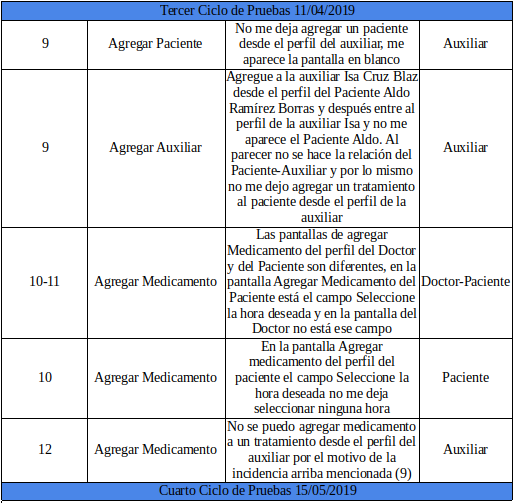
\includegraphics[height=0.8\textheight]{Pruebas/images/Inc3y4}
%		\caption{Incidencias}
%		\label{fig:Incidencias2}
%	\end{center}
%\end{figure}
%\newpage
\section{Pruebas de Usuario}

Al termino del desarrollo del Asistente Móvil para el Seguimiento de Tratamientos Médicos (Rem-Pills) se realizaron sesiones de prueba con Doctores, Pacientes y Auxiliares, para que conocieran la aplicación de Rem-Pills e interactuaran con ella.\\

El objetivo principal de las pruebas con los usuarios reales es conocer la opinión de ellos respecto al Asistente Móvil para el Seguimiento de Tratamientos Médicos (Rem-Pills), así como la evaluación que ellos nos daban respecto a su funcionamiento.\\

Después de que los usuarios reales interactuaran con la aplicación Rem-Pills nos interesó saber si ellos utilizarían Rem-Pills como apoyo para el seguimiento de los tratamientos médicos, por lo que se aplicó un cuestionario acerca de su opinión y funcionalidad de Rem-Pills.\\

Se realizaron un total de 12 pruebas de usabilidad y desempeño con usuarios distintos de los cuales 3 eran Doctores, 5 eran Pacientes y 4 eran padres de familia los cuales los consideramos como Auxiliares.\\

Los resultados que obtuvimos de las pruebas de usuario se muestran a continuación:\\

De los \textbf{Doctores} que probaron Rem-Pills:

\begin{itemize}
	\item A 2 de 3 doctores que realizaron las pruebas les pareció útil nuestra aplicación.
	\newpage
	\begin{figure}[htb]
		\centering
		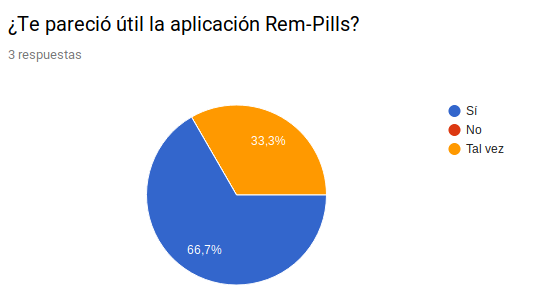
\includegraphics[width=0.7\textwidth]{images/Pruebas/Doc1}
		\caption{Cuestionario Rem-Pills} 
		\label{fig:Doc1}
	\end{figure} 
%	 
	\item 2 de 3 doctores piensan que utilizar nuestro asistente médico móvil (Rem-Pills) puede ayudar a tener más probabilidades de que sus pacientes terminen sus tratamientos médicos y el otro doctor puso que tal vez.
	\begin{figure}[htb]
		\centering
		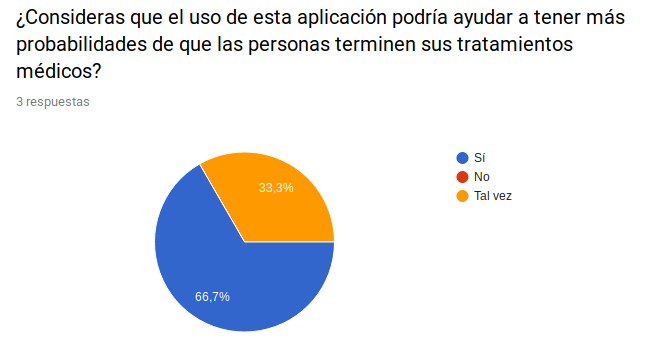
\includegraphics[width=0.7\textwidth]{images/Pruebas/Doc2}
		\caption{Cuestionario Rem-Pills} 
		\label{fig:Doc2}
	\end{figure} 
	
	
	\item 2 de 3 doctores piensan que la aplicación Rem-Pills es un buen asistente médico y si podrían comenzar a utilizarla con sus pacientes.
	\newpage
	\begin{figure}[htb]
		\centering
		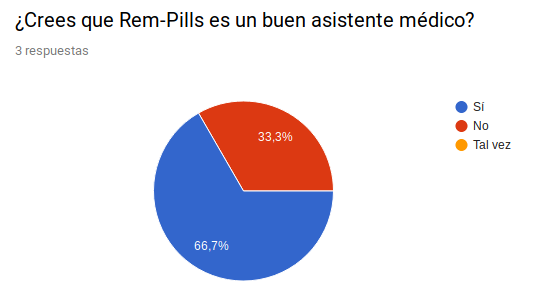
\includegraphics[width=0.7\textwidth]{images/Pruebas/Doc4}
		\caption{Cuestionario Rem-Pills} 
		\label{fig:Doc4}
	\end{figure} 
%	
%	
\end{itemize}
%\newpage
De los \textbf{Pacientes} que probaron Rem-Pills:

\begin{itemize}
	\item A 4 de 5 pacientes que realizaron las pruebas les pareció útil nuestra aplicación.

	\begin{figure}[htb]
		\centering
		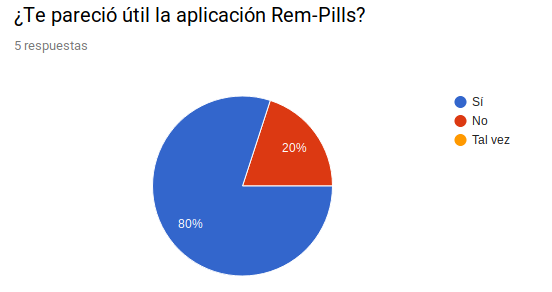
\includegraphics[width=0.7\textwidth]{images/Pruebas/Pac1}
		\caption{Cuestionario Rem-Pills} 
		\label{fig:Pac1}
	\end{figure} 
\newpage
	\item 2 de 5 Pacientes piensa que utilizar nuestro asistente médico móvil (Rem-Pills) puede ayudar a tener más probabilidades de terminar sus tratamientos médicos y los otros 3 pacientes pusieron que tal vez.
	\begin{figure}[htb]
		\centering
		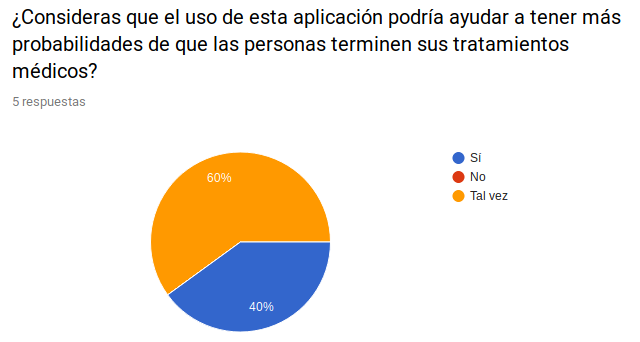
\includegraphics[width=0.7\textwidth]{images/Pruebas/Pac2}
		\caption{Cuestionario Rem-Pills} 
		\label{fig:Pac2}
	\end{figure} 

	
	\item 3 de 5 Pacientes piensan que utilizar nuestro asistente médico móvil (Rem-Pills) puede ayudar a recordar la hora de la toma de sus medicamentos y así mismo, a terminar sus tratamientos médicos satisfactoriamente y los otros 2 pusieron que tal vez.

	\begin{figure}[htb]
		\centering
		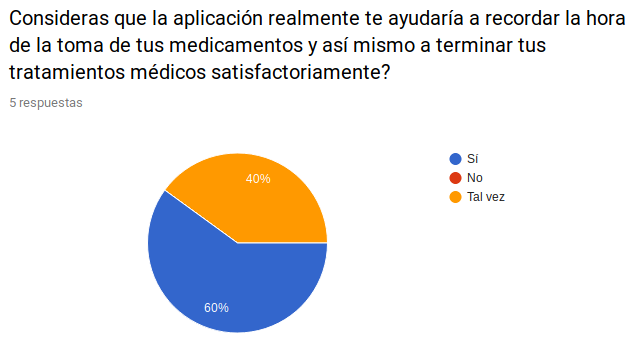
\includegraphics[width=0.7\textwidth]{images/Pruebas/Pac3}
		\caption{Cuestionario Rem-Pills} 
		\label{fig:Pac3}
	\end{figure} 
	\newpage
	\item 3 de 5 Pacientes piensan que la aplicación Rem-Pills es buena y si la utilizarían como asistente para el seguimiento de sus tratamientos médicos.
	\begin{figure}[htb]
		\centering
		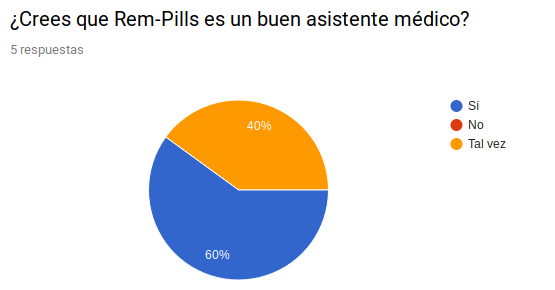
\includegraphics[width=0.7\textwidth]{images/Pruebas/Pac4}
		\caption{Cuestionario Rem-Pills} 
		\label{fig:Pac4}
	\end{figure} 
	
\end{itemize}
%\newpage
De los \textbf{Auxiliares} que probaron Rem-Pills:

\begin{itemize}
	
	\item 2 de 4 auxiliares que realizaron las pruebas piensa que utilizar nuestro asistente médico móvil (Rem-Pills) puede ayudar a tener más probabilidades de terminar sus tratamientos médicos y el otro puso que tal vez.
	
	\begin{figure}[htb]
		\centering
		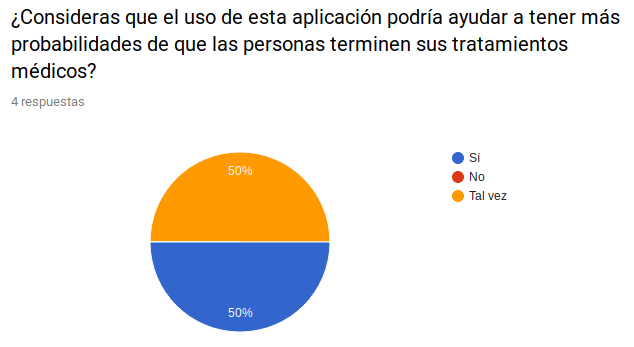
\includegraphics[width=0.7\textwidth]{images/Pruebas/Aux1}
		\caption{Cuestionario Rem-Pills} 
		\label{fig:Aux1}
	\end{figure} 
%%	
	\item Los 4 auxiliares que realizaron las pruebas piensan que utilizar nuestro asistente médico móvil (Rem-Pills) puede ayudar a recordar la hora de la toma de sus medicamentos y así mismo, a terminar sus tratamientos médicos satisfactoriamente.
	\newpage
	\begin{figure}[htb]
		\centering
		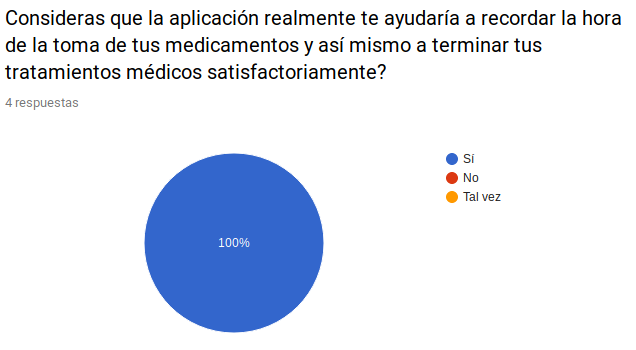
\includegraphics[width=0.7\textwidth]{images/Pruebas/Aux2}
		\caption{Cuestionario Rem-Pills} 
		\label{fig:Aux2}
	\end{figure} 
%	\newpage
	\item 3 de 4 auxiliares que realizaron las pruebas piensan que la aplicación Rem-Pills es buena y si la utilizarían como asistente para el seguimiento de sus tratamientos médicos.

	\begin{figure}[htb]
		\centering
		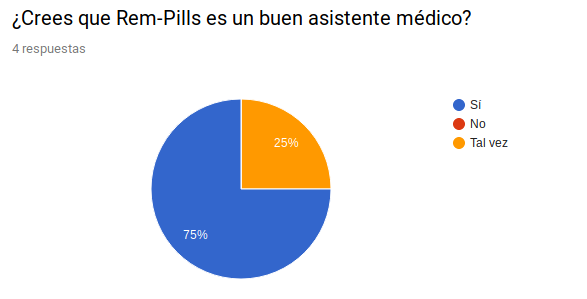
\includegraphics[width=0.7\textwidth]{images/Pruebas/Aux3}
		\caption{Cuestionario Rem-Pills} 
		\label{fig:Aux3}
	\end{figure} 
%	
\end{itemize}

Los cuestionarios que se realizaron a los usuarios que realizaron las pruebas a nuestra aplicación Rem-Pills son los siguientes:

\includepdf[pages=1-20]{Cuestionarios.pdf}
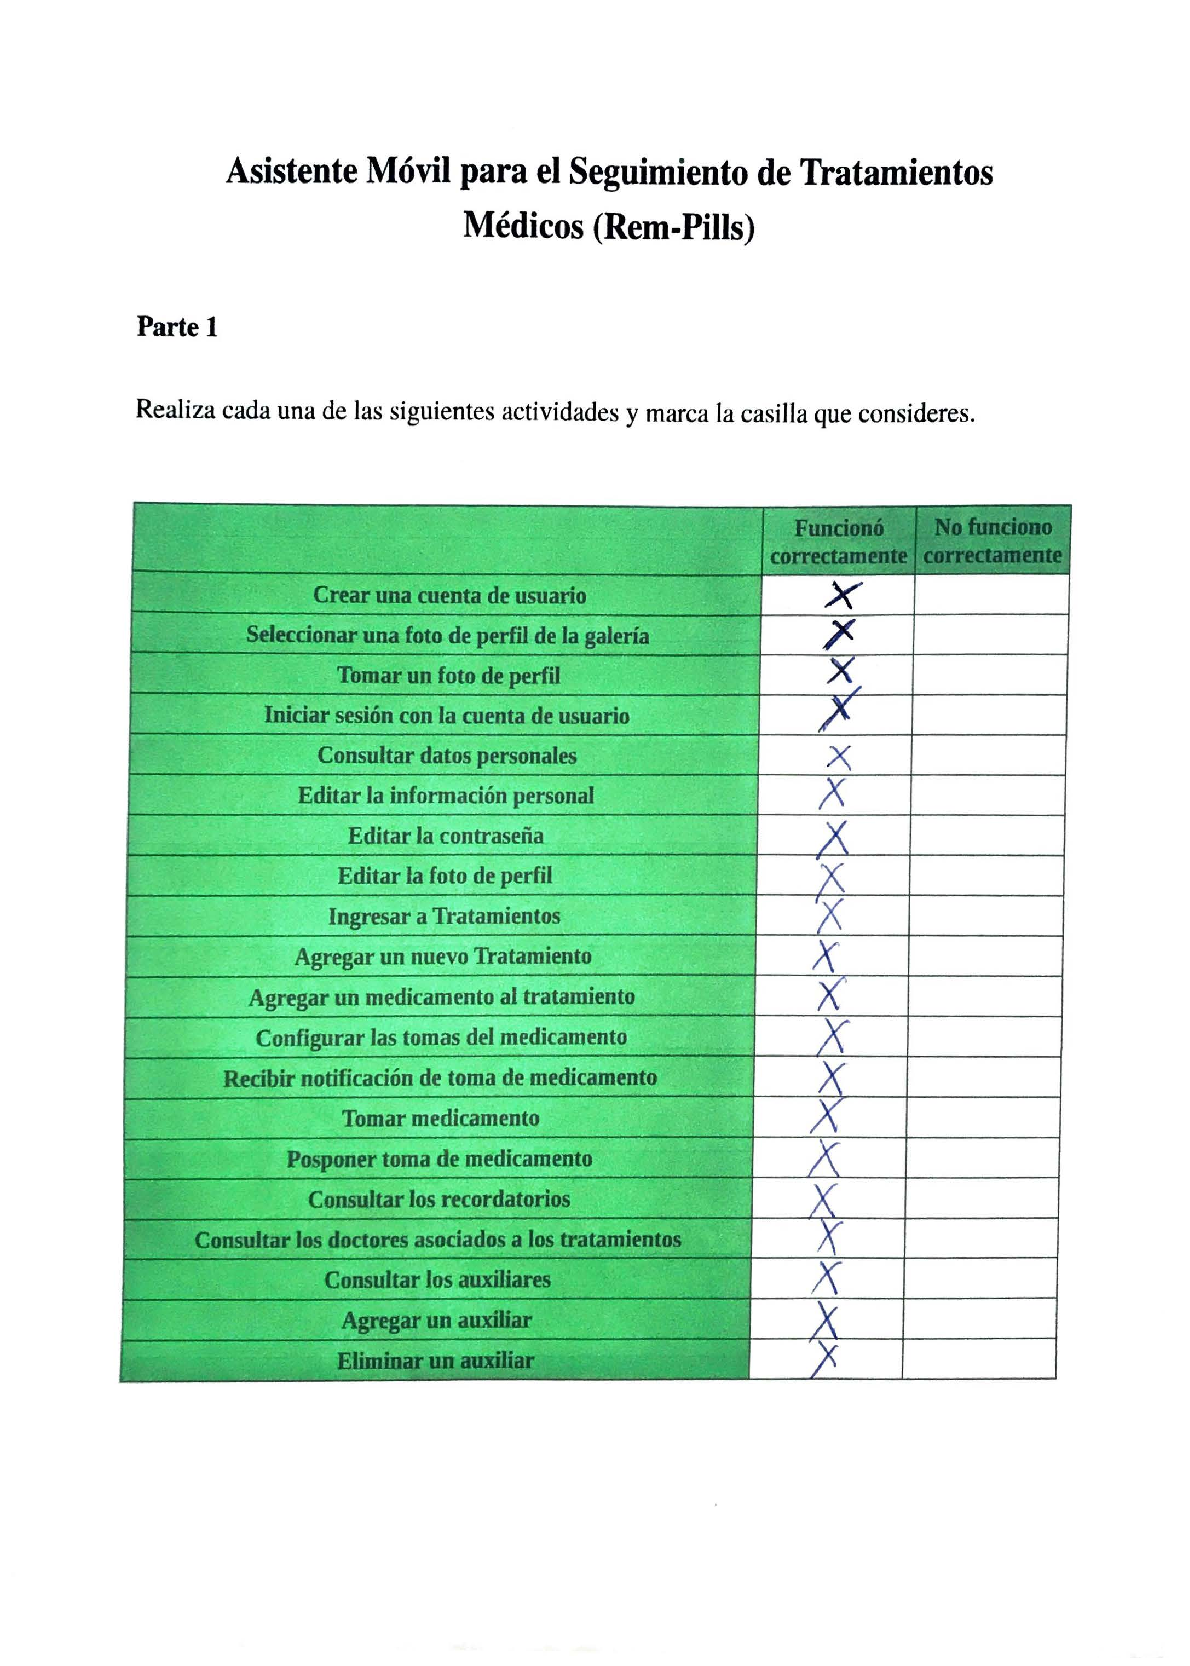
\includepdf[pages=1-4]{Cuestionarios2.pdf}

\newpage
Con estas pruebas de usuario realizadas podemos llegar a la conclusión de que nuestro asistente médico móvil (Rem-Pills) es una buena aplicación y si podría ayudar como asistente para el seguimiento de los tratamientos médicos de los usuarios.